\subsection{Test Case Experimental Setup and Offline Results}
Fig. \ref{fig:simulation_grid} shows the test system simulated for validating the effectiveness of the EMS. The simulated power system is the reduced feeder shown in Fig. \ref{fig:modelreduction} with one change. The section of the figure marked by the black dashed lines has been converted into a microgrid by adding ES with the PV system. Table \ref{tab:SYSTEM} shows the parameters of the PV and ES systems.
\begin{figure}[!ht]
    \centering
    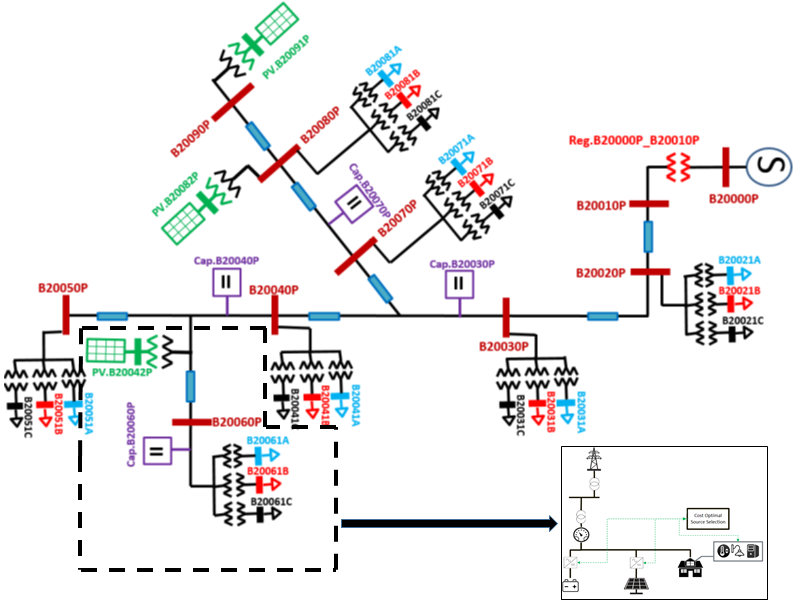
\includegraphics[width = \linewidth]{figs/simulation_grid.png}
    \caption{One line diagram of reduced distribution system for CHIL testing.}
    \label{fig:simulation_grid}
\end{figure}
%\vspace{-2mm}


\begin{table}[htb]
\caption{PV and ES system parameters}
\label{tab:SYSTEM}
\centering
\begin{tabular}{|c|c|c|}
\hline
\textbf{System parameter}            & \textbf{PV} & \textbf{ES} \\ \hline
Rated power                          & 875 kW      & 750 kW      \\ \hline
Inverter power rating                & 900 kVA     & 750 kVA     \\ \hline
Maximum cahrge                       & NA          & 2190 kWh    \\ \hline
Minimum charge                       & NA          & 219 kWh     \\ \hline
Levelized cost of electricity (LCOE) & 2.51 c/kWh  & 12.3 c/kWh  \\ \hline
\end{tabular}
\end{table}
%\vspace{-2mm}

The system is simulated in MATLAB\textsuperscript{\textregistered} Simulink\textsuperscript{\textregistered} using the Simscape Power Systems\textsuperscript{TM} toolbox in phasor domain for the Offline simulation. The A* based ESM is run, and the results are fed in as an open loop control to a Simulink model for phasor simulation. In the test cases, the  SOC of the ESS is discretized in steps of 2\%, and the SOC is limited between  94\%  and  10\%. The time-step and the control horizon chosen is 15 minutes. The ES is allowed to charge or discharge a maximum of 8\% of its total capacity during one time-step. The 8\% limitation is set based on the power specifications discussed in table \ref{tab:SYSTEM}. The A* search runs every 15 minutes considering a 24 hours (96 time-steps) prediction horizon. The PV and load profile used in the simulation are real data collected from the system shown in Fig. \ref{fig:modelreduction}. The price profile is based on real-time price data collected from the New York Independent System Operator (NYISO).


% \begin{figure}[!ht]
%     \centering
%     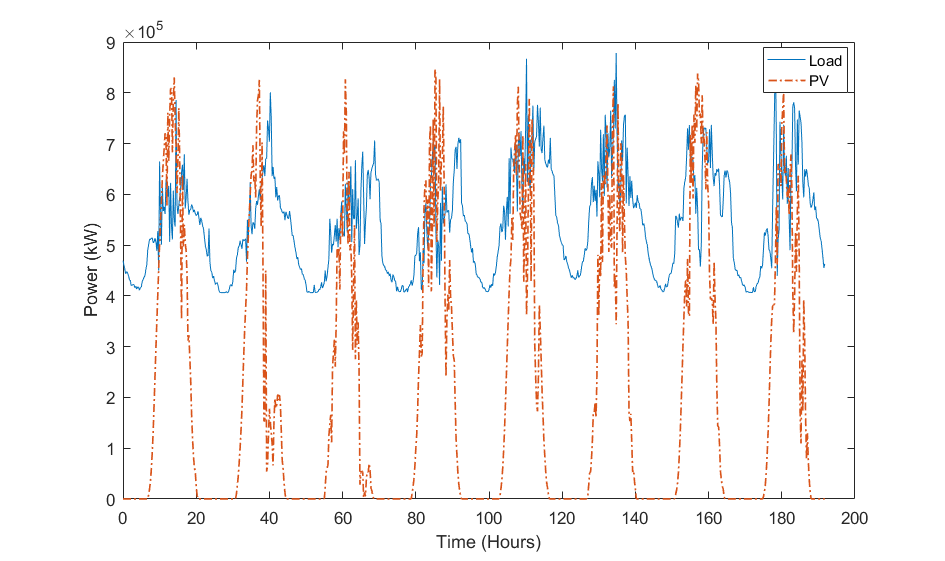
\includegraphics[width = \linewidth]{figs/PV_LOAD_PROF.png}
%     \caption{Eight day PV and load profile used in simulation.}
%     \label{fig:PV_LOAD_PROF}
% \end{figure}

% \begin{figure}[!ht]
%     \centering
%     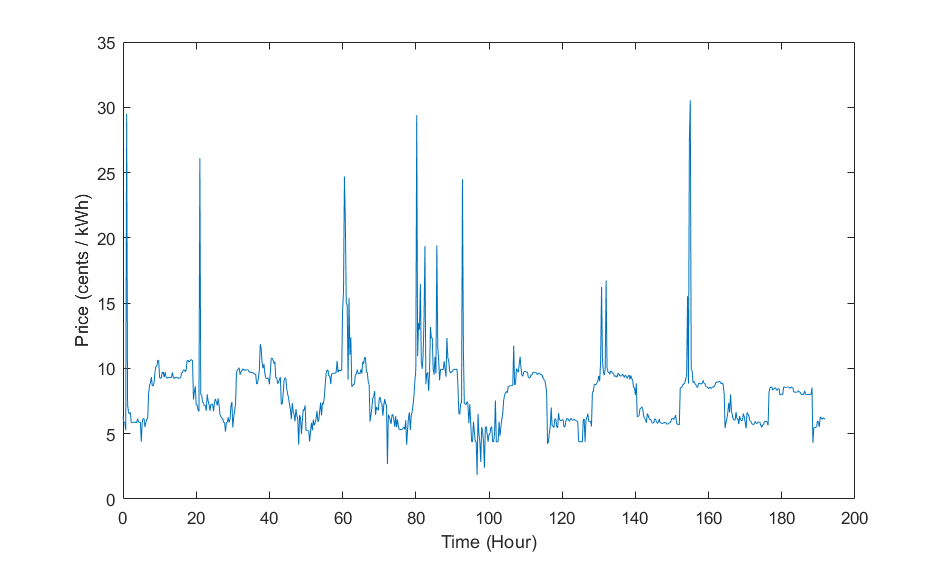
\includegraphics[width = \linewidth]{figs/RTP_NY.png}
%     \caption{Eight day price profile from NYISO.}
%     \label{fig:RTP_PROFILE_NY}
% \end{figure}

The performance of the algorithm is compared against genetic algorithm (GA) and sequential quadratic programming (SQP) algorithm approaches under a net metering scheme. Brief descriptions of the GA and SQP algorithms used are given below.
\begin{itemize}
    \item \textbf{GA case:} In this case, GA was used to find the minimum cost of (\ref{eq:C_actual}) in every time-step. The GA used a population size of 150. Increasing population size over this number did not show significant improvement and increased computation time significantly. The genetic algorithm solver available with MATLAB\textsuperscript{\textregistered} \cite{GA} was used to find the minimum cost of  (\ref{eq:C_actual}) while maintaining the ES charging and discharging constraints mentioned before (ES can charge and discharge a maximum of 8\% of total capacity and SOC is kept between 10\% to 94\%).
    
    \item \textbf{SQP case:} In this case SQP was used to find the minimum cost of (\ref{eq:C_actual}) in every time-step. The SQP solver available with fmincon in  MATLAB\textsuperscript{\textregistered} was used to obtain the minimum. The constraints for the SQP approach are the same as the GA approach.

\end{itemize}

Fig. \ref{fig:SBMPO_COMP_1_day} shows a zoomed view of the first day of the 7-day simulation for the A* based EMS. The solid black line in the figure represents the SOC of the energy storage, and the dotted red line represents the RTP. The dashed blue line represents the apparent demand. The left vertical axis of the graph represents the RTP of energy and the SOC of the ES. The right vertical axis represents the kWh apparent demand (actual demand - PV generation) of the system. A negative apparent demand represents excess energy from the local generation after fulfilling the local demand. The horizontal axis represents time in hours. The arrows with the numbers are showing specific points of the figure that are explained next, based on the behavior of the EMS. As observed in Fig. \ref{fig:SBMPO_COMP_1_day}, there are two peaks in price at points 1 and 3 throughout the 24 hours window of operation. The ESM accurately anticipates the price peak in point 1 and charges the energy storage using the grid just before the peak occurs, and discharges during the price peak at point 1. It can be seen that during the peak, the apparent demand was positive and the cheapest available price for grid energy was available just before the peak. The algorithm also anticipates the next price peak at point 3 based on forecasted data and prepares the ES to discharge at that price peak by charging at the lowest RTP period at point 2. Although, there is excess generation available from the PV in between point 2 and point 3, the opportunity cost of using the PV to charge the ES will be equal to the RTP due to net metering. So, in this case, the algorithm behaves as expected and uses the lowest possible RTP period to charge the ES and discharges during the price period when there is a high enough peak price to justify the use of the energy storage.
\begin{figure}[!ht]
    \centering
    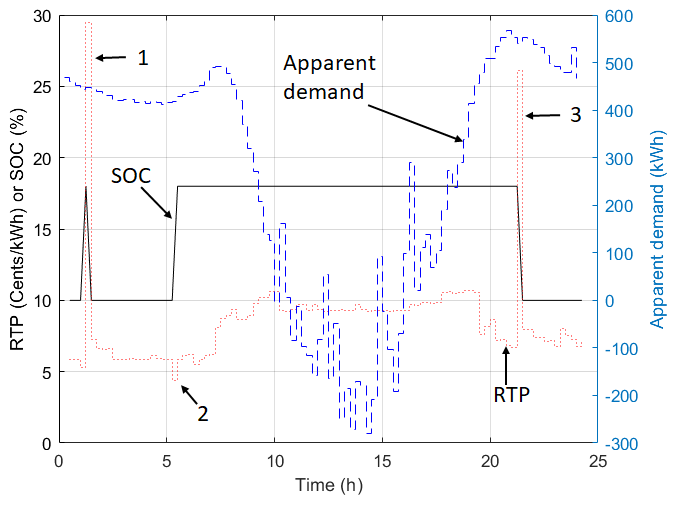
\includegraphics[width = \linewidth]{figs/SBMPO_COMP_1_day.png}
    \caption{First day EMS response for net metering comparison case}
    \label{fig:SBMPO_COMP_1_day}
\end{figure}
Fig. \ref{fig:SBMPO_COMP_10_12} shows the response of the A*-based EMS in a seven-day run used in the same microgrid system.  It can be seen from Fig. \ref{fig:SBMPO_COMP_10_12} that the A*-based ESM is following the same behavior displayed in Fig. \ref{fig:SBMPO_COMP_1_day}. It's taking advantage of the lowest energy price before a peak price appears in its prediction horizon, and charging the energy storage in order to discharge it when there is a high enough price peak. The total cost of operation for the A*-based ESM for the seven-day period is shown in Table \ref{tab:Cost1} and it can be seen that the method shows significant savings ranging from 5\% to 8.9\% depending on the case compared.

\begin{table}[htb]
\caption{Total cost for seven-day offline simulation}
\centering
\label{tab:Cost1}
\begin{tabular}{|l|l|}
\hline
GA Case & \$5,335 \\ \hline
SQP Case & \$5,117 \\ \hline
A* Case & \$4,861 \\ \hline
A* Case \% savings over GA Case & 8.9\% \\ \hline
A* Case \% savings over SQP Case & 5.0\% \\ \hline
\end{tabular}
\end{table}

\vspace{-2mm}

\begin{figure}[!ht]
    \centering
    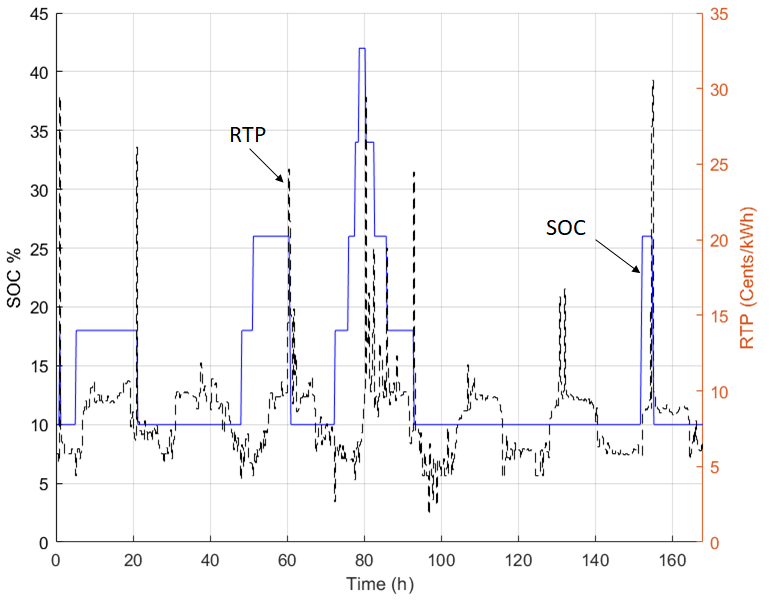
\includegraphics[width = \linewidth]{figs/SBMPO_COMP_10_12.png}
    \caption{Seven-day EMS response for off-line simulation}
    \label{fig:SBMPO_COMP_10_12}
    \vspace{-5mm}
\end{figure}

\subsection{\hl{Effects of discretization and time-step}}

Table \ref{tab:SIM_PER_1} \hl{shows the effects of discretization and time-step on the overall performance of the algorithm. It shows seven day test results with 2\%, 3\% \& 5\% discretization of the SOC of the energy storage for a time-steps of 10 minute, 30 minute \& 60 minute. It is evident from the table that increasing the time step and discretization levels results in faster execution time with a higher cost. While decreasing any of these properties increases execution time but also provides a better cost.}

\begin{table}[htb]
\caption{Effects of discretization and time-step on the algorithm performance}
\centering
\label{tab:SIM_PER_1}
\begin{tabular}{|l|l|l|l|}
\hline
\diagbox{Discretization}{Time-step} & 15 minute & 30 minute & 60 minute \\ \hline
2\% & \begin{tabular}[c]{@{}l@{}}Cost: \$4861\\ Time: 4s\end{tabular} & \begin{tabular}[c]{@{}l@{}}Cost: \$4871\\ Time: 2.1s\end{tabular} & \begin{tabular}[c]{@{}l@{}}Cost: \$4883\\ Time: 1.5s\end{tabular} \\ \hline
3\% & \begin{tabular}[c]{@{}l@{}}Cost: \$4893\\ Time: 2.9s\end{tabular} & \begin{tabular}[c]{@{}l@{}}Cost: \$4920\\ Time: 1.3s\end{tabular} & \begin{tabular}[c]{@{}l@{}}Cost: \$4951\\ Time: 0.9s\end{tabular} \\ \hline
5\% & \begin{tabular}[c]{@{}l@{}}Cost: \$4915\\ Time: 2.7s\end{tabular} & \begin{tabular}[c]{@{}l@{}}Cost: \$4970\\ Time: 1.1s\end{tabular} & \begin{tabular}[c]{@{}l@{}}Cost: \$5122\\ Time: 0.3s\end{tabular} \\ \hline
\end{tabular}
\end{table}

